\documentclass[10pt]{beamer}

% \usepackage{define}
\usepackage{animate}

\usetheme{CCFD}
\usepackage{color}
\definecolor{gray97}{gray}{.90}
\definecolor{gray75}{gray}{.75}
\usepackage{listings}
\lstset{frame=Ltb,
     framerule=0pt,
     aboveskip=0cm,
     framextopmargin=0pt,
     framexbottommargin=0pt,
     framexleftmargin=0cm,
     framesep=0pt,
     rulesep=0pt,
     backgroundcolor=\color{gray97},
     rulesepcolor=\color{black},
     language=C,
           basicstyle=\ttfamily\scriptsize,
           keywordstyle=\color{blue}\ttfamily,
           stringstyle=\color{red}\ttfamily,
           commentstyle=\color{green}\ttfamily,
          breaklines=true,
          }
\lstdefinestyle{consol}
   {basicstyle=\scriptsize\bf\ttfamily,
    backgroundcolor=\color{gray75},
}
\resetcounteronoverlays{lstnumber}

\newcommand{\tabitem}{%
  \usebeamertemplate{itemize item}\hspace*{\labelsep}}

\usepackage{tikz}
\usetikzlibrary{calc,shapes,arrows.meta}

\eventtitle{Computer Science I}
\title{Lecture 9\\2D Arrays\\{\tiny and examples}}
\date{}

\setbeamertemplate{blocks}[rounded][shadow=true]
\setbeamertemplate{navigation symbols}[]

\begin{document}

\frame{
    \titlepage
}

\section{2D arrays}

\begin{frame}[fragile]
  \frametitle{2D arrays}
  \framesubtitle{Declaration}
Syntax:
\begin{lstlisting}
type name[size 1][size 2]
\end{lstlisting}
\begin{itemize}
  \item \textit{type} - almost any type, pointer, etc.
  \item \textit{name} - an identifier
  \item \textit{size1} and \textit{size 2} - \textbf{MUST} be known at compilation time 
\end{itemize}
e.g.:
\begin{lstlisting}
//2x3 ints array of-> 6 ints -> 24B
int tabA[2][3];
//5x3 double array ->  15 doubles -> 120B
double tabB[5][3];
\end{lstlisting}
\begin{itemize}
  \item Continous in memory
  \item Occupies \textit{size 1} x \textit{size 2} x \textit{sizeof(type)} B
  \item Acces elements with double \textit{[]}, e.g.: \textit{tab[i][j]}
\end{itemize}
\begin{lstlisting}
tabA[0][0] // first row first column
tabA[0][2] // first row third column
tabA[1][2] // second row third column
\end{lstlisting}
\end{frame}

\subsection{Mamory}

\begin{frame}[fragile]
  \frametitle{2D arrays}
  \framesubtitle{Memory}
  \vspace{-0.3cm}
  \begin{columns}
    \begin{column}{0.65\textwidth}
      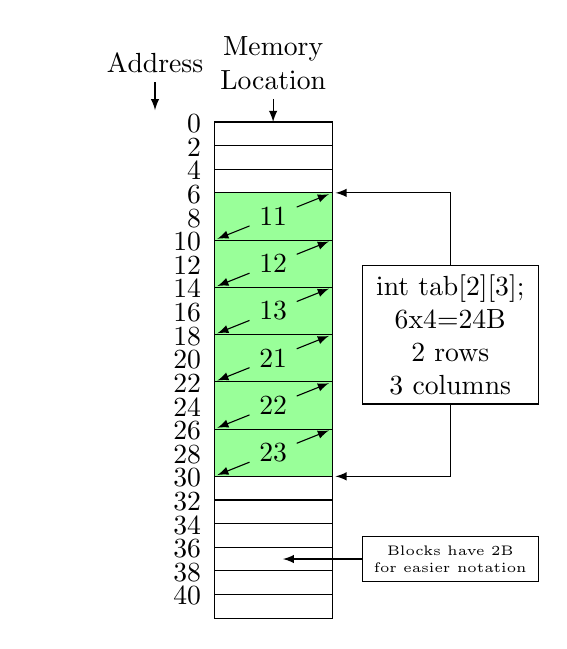
\begin{tikzpicture}[x=1.5cm,y=0.3cm]
  %% Building the boxes representing memory locations
  \foreach \x in {0,1,...,20}
  {
    \node[inner sep=1pt] (BL\x) at (0,-\x)   {};
    \node[inner sep=1pt] (UR\x) at (1,-\x+1) {};
    \node (MM\x) at ($(BL\x)!0.5!(UR\x)$) {};
    \draw (BL\x) rectangle (UR\x);
    \edef\memoryNumber{\number\numexpr0+2*\x}
    \node[anchor=south east] at (BL\x.north west) {\memoryNumber};
  }

  %% Label columns:
  \node (MEMLOC) at ($(MM0)+(0.0,0.9cm)$) { \parbox{2cm}{\centering Memory Location} };
  \node (ADDRESS) at ($(MEMLOC)-(1.0,0)$) {\parbox{3cm}{\centering Address} };
  \draw [-latex] (MEMLOC) -- ($(MM0|-UR0)+(0.0,0)$);
  \draw [-latex] (ADDRESS) -- ($(MM0|-UR0)-(1,-0.5)$);

  \foreach \x/\y in {4/3}
  {
    \draw[fill=green!40] (BL\x) rectangle (UR\y);
    \node (M\x-\y) at ($(BL\x)!0.5!(UR\y)$) {11};
    \draw[-latex]  (M\x-\y) -- (BL\x) ;
    \draw[-latex]  (M\x-\y) -- (UR\y) ;
  }
  \foreach \x/\y in {6/5}
  {
    \draw[fill=green!40] (BL\x) rectangle (UR\y);
    \node (M\x-\y) at ($(BL\x)!0.5!(UR\y)$) {12};
    \draw[-latex]  (M\x-\y) -- (BL\x) ; 
    \draw[-latex]  (M\x-\y) -- (UR\y) ;
  }
  \foreach \x/\y in {8/7}
  {
    \draw[fill=green!40] (BL\x) rectangle (UR\y);
    \node (M\x-\y) at ($(BL\x)!0.5!(UR\y)$) {13};
    \draw[-latex]  (M\x-\y) -- (BL\x) ; 
    \draw[-latex]  (M\x-\y) -- (UR\y) ;
  }
  \foreach \x/\y in {10/9}
  {
    \draw[fill=green!40] (BL\x) rectangle (UR\y);
    \node (M\x-\y) at ($(BL\x)!0.5!(UR\y)$) {21};
    \draw[-latex]  (M\x-\y) -- (BL\x) ; 
    \draw[-latex]  (M\x-\y) -- (UR\y) ;
  }
  \foreach \x/\y in {12/11}
  {
    \draw[fill=green!40] (BL\x) rectangle (UR\y);
    \node (M\x-\y) at ($(BL\x)!0.5!(UR\y)$) {22};
    \draw[-latex]  (M\x-\y) -- (BL\x) ; 
    \draw[-latex]  (M\x-\y) -- (UR\y) ;
  }
  \foreach \x/\y in {14/13}
  {
    \draw[fill=green!40] (BL\x) rectangle (UR\y);
    \node (M\x-\y) at ($(BL\x)!0.5!(UR\y)$) {23};
    \draw[-latex]  (M\x-\y) -- (BL\x) ; 
    \draw[-latex]  (M\x-\y) -- (UR\y) ;
  }
  
  \foreach \x/\y in {15/3}
  {
    \node[draw] (M\x-\y) at ($0.5*(UR\x)+0.5*(UR\y)+(1,0)$)
    { \parbox{2cm}{\centering int tab[2][3];\\6x4=24B\\2 rows\\3 columns}};
    \draw[-latex]  (M\x-\y) |- (UR\x) ; 
    \draw[-latex]  (M\x-\y) |- (UR\y) ;
  }

    \node[draw] (M18) at ($(MM18)+(1.5,0)$)
    { \parbox{2cm}{\centering \tiny Blocks have 2B\\for easier notation}};
    \draw[-latex]  (M18) -- (MM18) ; 

\end{tikzpicture}
    \end{column}
    \begin{column}{0.5\textwidth}
      \begin{itemize}
        \item Indexing is from 0 to size-1
        \item Storage is row based
        \item Array is stored row after row
      \end{itemize}
Example:
\begin{lstlisting}
int tab[2][3];

tab[0][0]=11;
tab[0][1]=12;
tab[0][2]=13;

tab[1][0]=21;
tab[1][1]=22;
tab[1][2]=23;
\end{lstlisting}
\centering   
\begin{tikzpicture}
    \matrix[matrix of nodes,nodes={draw}] {
      11 & 12 & 13 \\
      21 & 22 & 23 \\
    };
\end{tikzpicture}

    \end{column}
  \end{columns}
\end{frame}

\begin{frame}[fragile]
  \frametitle{2D arrays}
  \framesubtitle{Memory}
  \vspace{-0.3cm}
  \begin{columns}
    \begin{column}{0.65\textwidth}
      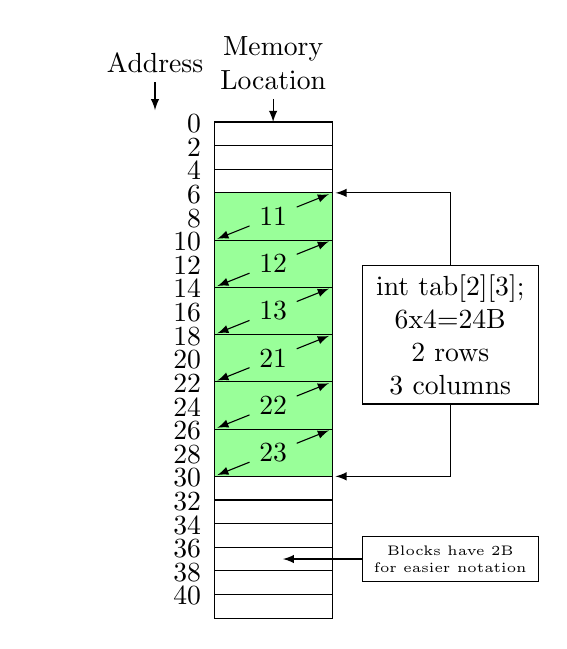
\begin{tikzpicture}[x=1.5cm,y=0.3cm]
  %% Building the boxes representing memory locations
  \foreach \x in {0,1,...,20}
  {
    \node[inner sep=1pt] (BL\x) at (0,-\x)   {};
    \node[inner sep=1pt] (UR\x) at (1,-\x+1) {};
    \node (MM\x) at ($(BL\x)!0.5!(UR\x)$) {};
    \draw (BL\x) rectangle (UR\x);
    \edef\memoryNumber{\number\numexpr0+2*\x}
    \node[anchor=south east] at (BL\x.north west) {\memoryNumber};
  }

  %% Label columns:
  \node (MEMLOC) at ($(MM0)+(0.0,0.9cm)$) { \parbox{2cm}{\centering Memory Location} };
  \node (ADDRESS) at ($(MEMLOC)-(1.0,0)$) {\parbox{3cm}{\centering Address} };
  \draw [-latex] (MEMLOC) -- ($(MM0|-UR0)+(0.0,0)$);
  \draw [-latex] (ADDRESS) -- ($(MM0|-UR0)-(1,-0.5)$);

  \foreach \x/\y in {4/3}
  {
    \draw[fill=green!40] (BL\x) rectangle (UR\y);
    \node (M\x-\y) at ($(BL\x)!0.5!(UR\y)$) {11};
    \draw[-latex]  (M\x-\y) -- (BL\x) ;
    \draw[-latex]  (M\x-\y) -- (UR\y) ;
  }
  \foreach \x/\y in {6/5}
  {
    \draw[fill=green!40] (BL\x) rectangle (UR\y);
    \node (M\x-\y) at ($(BL\x)!0.5!(UR\y)$) {12};
    \draw[-latex]  (M\x-\y) -- (BL\x) ; 
    \draw[-latex]  (M\x-\y) -- (UR\y) ;
  }
  \foreach \x/\y in {8/7}
  {
    \draw[fill=green!40] (BL\x) rectangle (UR\y);
    \node (M\x-\y) at ($(BL\x)!0.5!(UR\y)$) {13};
    \draw[-latex]  (M\x-\y) -- (BL\x) ; 
    \draw[-latex]  (M\x-\y) -- (UR\y) ;
  }
  \foreach \x/\y in {10/9}
  {
    \draw[fill=green!40] (BL\x) rectangle (UR\y);
    \node (M\x-\y) at ($(BL\x)!0.5!(UR\y)$) {21};
    \draw[-latex]  (M\x-\y) -- (BL\x) ; 
    \draw[-latex]  (M\x-\y) -- (UR\y) ;
  }
  \foreach \x/\y in {12/11}
  {
    \draw[fill=green!40] (BL\x) rectangle (UR\y);
    \node (M\x-\y) at ($(BL\x)!0.5!(UR\y)$) {22};
    \draw[-latex]  (M\x-\y) -- (BL\x) ; 
    \draw[-latex]  (M\x-\y) -- (UR\y) ;
  }
  \foreach \x/\y in {14/13}
  {
    \draw[fill=green!40] (BL\x) rectangle (UR\y);
    \node (M\x-\y) at ($(BL\x)!0.5!(UR\y)$) {23};
    \draw[-latex]  (M\x-\y) -- (BL\x) ; 
    \draw[-latex]  (M\x-\y) -- (UR\y) ;
  }
  
  \foreach \x/\y in {15/3}
  {
    \node[draw] (M\x-\y) at ($0.5*(UR\x)+0.5*(UR\y)+(1,0)$)
    { \parbox{2cm}{\centering int tab[2][3];\\6x4=24B\\2 rows\\3 columns}};
    \draw[-latex]  (M\x-\y) |- (UR\x) ; 
    \draw[-latex]  (M\x-\y) |- (UR\y) ;
  }

    \node[draw] (M18) at ($(MM18)+(1.5,0)$)
    { \parbox{2cm}{\centering \tiny Blocks have 2B\\for easier notation}};
    \draw[-latex]  (M18) -- (MM18) ; 

\end{tikzpicture}
    \end{column}
    \begin{column}{0.5\textwidth}
    \begin{enumerate}
      \item Write a program using a 2D static array.
      \item Access elements using \textit{[]}.
      \item Print an address of each array element using \&tab[i][j].
      \item What is a distance of:
      \begin{itemize}
        \item tab[i][j] and tab[i+1][j]
        \item tab[i][j] and tab[i][j+1]
      \end{itemize}
      \item Can a 2D array be treated as 1D?
      \item Consequences?
    \end{enumerate}

    \end{column}
  \end{columns}
\end{frame}

\subsection{2D arrays and functions}

\begin{frame}[fragile]
  \frametitle{2D arrays}
  \framesubtitle{Functions}
  \begin{itemize}
    \item Defining a function:
\begin{lstlisting}
type function_name(array_type tab[][SIZE2], ...)
{
  //Function body
}
\end{lstlisting}
\item Usage:
\begin{lstlisting}
array_type tab[SIZE1][SIZE2];
...
//Call the function, pass an array as an argument
function_name(tab, ...); 
\end{lstlisting}
  
\item The second bracket \textbf{MUST} give the size of an array.
\item Function is compiled separately
\item Changing the second index moves to the next memory block
\item Changing the first index moves us to the next row.
\item The size of row must be known!
\item See previous example!
\end{itemize}

\end{frame}

\begin{frame}[fragile]
  \frametitle{2D arrays}
  \framesubtitle{Examples}

\begin{enumerate}
	\item Write a program illustrating workings of a 2D static array
	\item Add initialization function
	\item Distinguish the maximum size of an array, and the one used by the program
	\item Illustrate how to write functions with 2D arrays
	\item Add a function printing a 2D array
	\item Add a function coping to a 1D vector the diagonal from a square matrix
	\item Write a function coping a row, column from a 2D array
	\item Write a function inserting a row column into a 2D array
\end{enumerate}

\end{frame}

\section{Dynamic memory allocation}

\begin{frame}[fragile]
  \frametitle{Dynamic memory allocation}
\centering
We know how to declare static arrays. We need a method to deal with situations when the size of an array is unknown at compilation time.

C offers \textit{malloc}, located in stdlib.h

\begin{lstlisting}
void* malloc (size_t size);
void* malloc (unsigned int size);
\end{lstlisting}

\begin{enumerate}
	\item Allocates a block of \textbf{\textit{size}} bytes of memory
	\item Returns a pointer to the beginning of that block
	\item The content allocated block of memory is not initialized
	\item \textit{size t} is \textit{unsigned int}
	\item For each malloc there needs to be a single \textit{free}
\begin{lstlisting}
type * p = (type*)malloc(size);
free(p)
\end{lstlisting}
	\item \textbf{After} we are done with using the memory

\end{enumerate}


\end{frame}

\begin{frame}[fragile]
  \frametitle{Dynamic memory allocation}
  \vspace{-0.3cm}
  \begin{columns}
    \begin{column}{0.65\textwidth}
      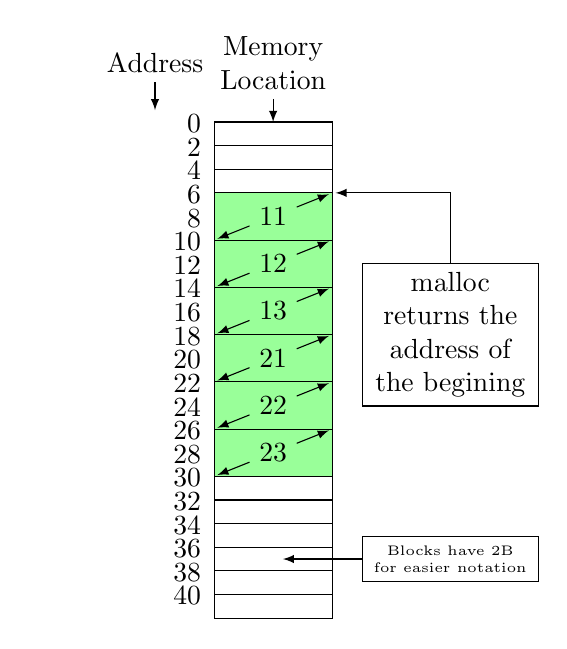
\begin{tikzpicture}[x=1.5cm,y=0.3cm]
  %% Building the boxes representing memory locations
  \foreach \x in {0,1,...,20}
  {
    \node[inner sep=1pt] (BL\x) at (0,-\x)   {};
    \node[inner sep=1pt] (UR\x) at (1,-\x+1) {};
    \node (MM\x) at ($(BL\x)!0.5!(UR\x)$) {};
    \draw (BL\x) rectangle (UR\x);
    \edef\memoryNumber{\number\numexpr0+2*\x}
    \node[anchor=south east] at (BL\x.north west) {\memoryNumber};
  }

  %% Label columns:
  \node (MEMLOC) at ($(MM0)+(0.0,0.9cm)$) { \parbox{2cm}{\centering Memory Location} };
  \node (ADDRESS) at ($(MEMLOC)-(1.0,0)$) {\parbox{3cm}{\centering Address} };
  \draw [-latex] (MEMLOC) -- ($(MM0|-UR0)+(0.0,0)$);
  \draw [-latex] (ADDRESS) -- ($(MM0|-UR0)-(1,-0.5)$);

  \foreach \x/\y in {4/3}
  {
    \draw[fill=green!40] (BL\x) rectangle (UR\y);
    \node (M\x-\y) at ($(BL\x)!0.5!(UR\y)$) {11};
    \draw[-latex]  (M\x-\y) -- (BL\x) ;
    \draw[-latex]  (M\x-\y) -- (UR\y) ;
  }
  \foreach \x/\y in {6/5}
  {
    \draw[fill=green!40] (BL\x) rectangle (UR\y);
    \node (M\x-\y) at ($(BL\x)!0.5!(UR\y)$) {12};
    \draw[-latex]  (M\x-\y) -- (BL\x) ; 
    \draw[-latex]  (M\x-\y) -- (UR\y) ;
  }
  \foreach \x/\y in {8/7}
  {
    \draw[fill=green!40] (BL\x) rectangle (UR\y);
    \node (M\x-\y) at ($(BL\x)!0.5!(UR\y)$) {13};
    \draw[-latex]  (M\x-\y) -- (BL\x) ; 
    \draw[-latex]  (M\x-\y) -- (UR\y) ;
  }
  \foreach \x/\y in {10/9}
  {
    \draw[fill=green!40] (BL\x) rectangle (UR\y);
    \node (M\x-\y) at ($(BL\x)!0.5!(UR\y)$) {21};
    \draw[-latex]  (M\x-\y) -- (BL\x) ; 
    \draw[-latex]  (M\x-\y) -- (UR\y) ;
  }
  \foreach \x/\y in {12/11}
  {
    \draw[fill=green!40] (BL\x) rectangle (UR\y);
    \node (M\x-\y) at ($(BL\x)!0.5!(UR\y)$) {22};
    \draw[-latex]  (M\x-\y) -- (BL\x) ; 
    \draw[-latex]  (M\x-\y) -- (UR\y) ;
  }
  \foreach \x/\y in {14/13}
  {
    \draw[fill=green!40] (BL\x) rectangle (UR\y);
    \node (M\x-\y) at ($(BL\x)!0.5!(UR\y)$) {23};
    \draw[-latex]  (M\x-\y) -- (BL\x) ; 
    \draw[-latex]  (M\x-\y) -- (UR\y) ;
  }
  
  \foreach \x/\y in {15/3}
  {
    \node[draw] (M\x-\y) at ($0.5*(UR\x)+0.5*(UR\y)+(1,0)$)
    { \parbox{2cm}{\centering malloc returns the address of the begining}};
      \draw[-latex]  (M\x-\y) |- (UR\y) ;
  }

    \node[draw] (M18) at ($(MM18)+(1.5,0)$)
    { \parbox{2cm}{\centering \tiny Blocks have 2B\\for easier notation}};
    \draw[-latex]  (M18) -- (MM18) ; 

\end{tikzpicture}
    \end{column}
    \begin{column}{0.55\textwidth}
      \begin{itemize}
        \item Indexing is from 0 to size-1
        \item Just like the 1D static one
      \end{itemize}
Example:
\begin{lstlisting}
int *p=(int*)malloc(24);

p[0] = 11;
p[1] = 12;
p[2] = 13;
p[3] = 21;
p[4] = 22;
p[5] = 23;

free(p);
\end{lstlisting}

    \end{column}
  \end{columns}
\end{frame}

\begin{frame}[fragile]
  \frametitle{Dynamic memory allocation}
  \framesubtitle{use \textit{sizeof()}}
  \vspace{-0.3cm}
  \begin{columns}
    \begin{column}{0.65\textwidth}
      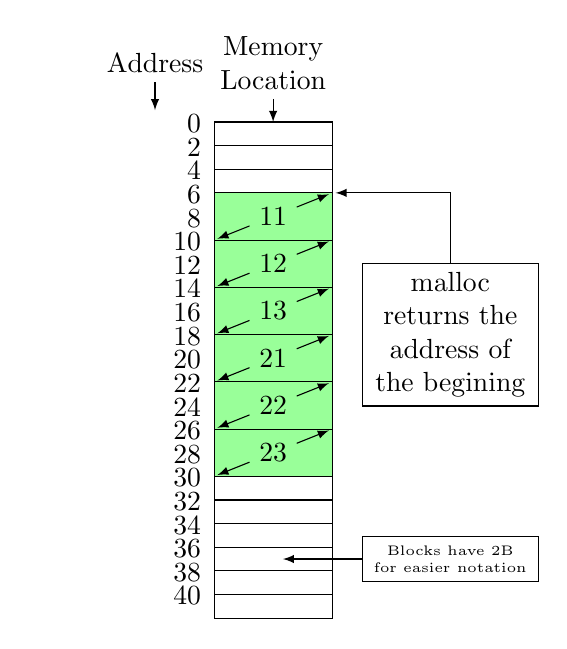
\begin{tikzpicture}[x=1.5cm,y=0.3cm]
  %% Building the boxes representing memory locations
  \foreach \x in {0,1,...,20}
  {
    \node[inner sep=1pt] (BL\x) at (0,-\x)   {};
    \node[inner sep=1pt] (UR\x) at (1,-\x+1) {};
    \node (MM\x) at ($(BL\x)!0.5!(UR\x)$) {};
    \draw (BL\x) rectangle (UR\x);
    \edef\memoryNumber{\number\numexpr0+2*\x}
    \node[anchor=south east] at (BL\x.north west) {\memoryNumber};
  }

  %% Label columns:
  \node (MEMLOC) at ($(MM0)+(0.0,0.9cm)$) { \parbox{2cm}{\centering Memory Location} };
  \node (ADDRESS) at ($(MEMLOC)-(1.0,0)$) {\parbox{3cm}{\centering Address} };
  \draw [-latex] (MEMLOC) -- ($(MM0|-UR0)+(0.0,0)$);
  \draw [-latex] (ADDRESS) -- ($(MM0|-UR0)-(1,-0.5)$);

  \foreach \x/\y in {4/3}
  {
    \draw[fill=green!40] (BL\x) rectangle (UR\y);
    \node (M\x-\y) at ($(BL\x)!0.5!(UR\y)$) {11};
    \draw[-latex]  (M\x-\y) -- (BL\x) ;
    \draw[-latex]  (M\x-\y) -- (UR\y) ;
  }
  \foreach \x/\y in {6/5}
  {
    \draw[fill=green!40] (BL\x) rectangle (UR\y);
    \node (M\x-\y) at ($(BL\x)!0.5!(UR\y)$) {12};
    \draw[-latex]  (M\x-\y) -- (BL\x) ; 
    \draw[-latex]  (M\x-\y) -- (UR\y) ;
  }
  \foreach \x/\y in {8/7}
  {
    \draw[fill=green!40] (BL\x) rectangle (UR\y);
    \node (M\x-\y) at ($(BL\x)!0.5!(UR\y)$) {13};
    \draw[-latex]  (M\x-\y) -- (BL\x) ; 
    \draw[-latex]  (M\x-\y) -- (UR\y) ;
  }
  \foreach \x/\y in {10/9}
  {
    \draw[fill=green!40] (BL\x) rectangle (UR\y);
    \node (M\x-\y) at ($(BL\x)!0.5!(UR\y)$) {21};
    \draw[-latex]  (M\x-\y) -- (BL\x) ; 
    \draw[-latex]  (M\x-\y) -- (UR\y) ;
  }
  \foreach \x/\y in {12/11}
  {
    \draw[fill=green!40] (BL\x) rectangle (UR\y);
    \node (M\x-\y) at ($(BL\x)!0.5!(UR\y)$) {22};
    \draw[-latex]  (M\x-\y) -- (BL\x) ; 
    \draw[-latex]  (M\x-\y) -- (UR\y) ;
  }
  \foreach \x/\y in {14/13}
  {
    \draw[fill=green!40] (BL\x) rectangle (UR\y);
    \node (M\x-\y) at ($(BL\x)!0.5!(UR\y)$) {23};
    \draw[-latex]  (M\x-\y) -- (BL\x) ; 
    \draw[-latex]  (M\x-\y) -- (UR\y) ;
  }
  
  \foreach \x/\y in {15/3}
  {
    \node[draw] (M\x-\y) at ($0.5*(UR\x)+0.5*(UR\y)+(1,0)$)
    { \parbox{2cm}{\centering malloc returns the address of the begining}};
      \draw[-latex]  (M\x-\y) |- (UR\y) ;
  }

    \node[draw] (M18) at ($(MM18)+(1.5,0)$)
    { \parbox{2cm}{\centering \tiny Blocks have 2B\\for easier notation}};
    \draw[-latex]  (M18) -- (MM18) ; 

\end{tikzpicture}
    \end{column}
    \begin{column}{0.55\textwidth}
      \begin{itemize}
        \item \textit{sizeof()} gives us the size of type
        \item 
      \end{itemize}
Example:
\begin{lstlisting}
int *p=(int*)malloc(6*sizeof(int));

p[0] = 11;
p[1] = 12;
p[2] = 13;
p[3] = 21;
p[4] = 22;
p[5] = 23;

free(p);
\end{lstlisting}

    \end{column}
  \end{columns}
\end{frame}

\begin{frame}[fragile]
  \frametitle{Dynamic memory allocation}
  \framesubtitle{With size from keyboard}
      \begin{itemize}
        \item Read the size from keyboard
        \item Allocate memory using \textit{malloc()}
      \end{itemize}

\begin{lstlisting}
int n;
scanf("%d", &n);
int *p=(int*)malloc(n*sizeof(int));

p[0] = 11;
p[1] = 12;
p[2] = 13;
p[3] = 21;
p[4] = 22;
p[5] = 23;

free(p);
\end{lstlisting}

      \begin{itemize}
        \item Recall the example with reading in array data from a file
        \item Read the size from file, allocate, read data ...
      \end{itemize}

\end{frame}

\begin{frame}[fragile]
  \frametitle{Dynamic memory allocation}
  \framesubtitle{Use with functions and compatibility with static arrays}
      \begin{itemize}
        \item In the case of 1D arrays it is the same as with static ones
        \item Example with bubble sorting
      \end{itemize}

\end{frame}

\begin{frame}[fragile]
  \frametitle{Dynamic memory allocation}
  \framesubtitle{Allocation of 2D arrays is a bit more complicated ...}
		Which we will find out next week
\end{frame}

\end{document}
